\documentclass[12pt,a4paper]{article}
\usepackage[utf8]{inputenc}
\usepackage[T1]{fontenc}
\usepackage{geometry}
\usepackage{graphicx}
\usepackage{float}
\usepackage{listings}
\usepackage{xcolor}
\usepackage{hyperref}
\usepackage{amsmath}
\usepackage{amsfonts}
\usepackage{amssymb}
\usepackage{tikz}
\usepackage{pgfplots}
\usepackage{booktabs}
\usepackage{longtable}
\usepackage{array}
\usepackage{multirow}
\usepackage{wrapfig}
\usepackage{rotating}
\usepackage{caption}
\usepackage{subcaption}
\usepackage{fancyhdr}
\usepackage{enumitem}
\usepackage{setspace}

% Page setup
\geometry{margin=1in}
\pagestyle{fancy}
\fancyhf{}
\rhead{Big Data Research System}
\lhead{Technical Report}
\rfoot{Page \thepage}

% Code listing setup
\lstset{
    basicstyle=\ttfamily\footnotesize,
    breaklines=true,
    frame=single,
    numbers=left,
    numberstyle=\tiny,
    keywordstyle=\color{blue},
    commentstyle=\color{green!60!black},
    stringstyle=\color{red},
    backgroundcolor=\color{gray!10},
    showstringspaces=false
}

% Title page
\title{\Huge\textbf{Big Data Research System}\\[0.5cm]
\Large A Comprehensive Data Pipeline for COVID-19 Research Analysis}
\author{Technical Report}
\date{\today}

\begin{document}

\maketitle
\thispagestyle{empty}

\newpage
\tableofcontents
\newpage

\section{Executive Summary}

This report presents a comprehensive analysis of the Big Data Research System, a sophisticated data pipeline designed for collecting, processing, and analyzing COVID-19 related research data from multiple heterogeneous sources. The system implements a modern big data architecture utilizing cutting-edge technologies including Apache Airflow, Apache Kafka, Apache Spark, Apache Hadoop (HDFS), PostgreSQL, and dbt for data transformation.

The primary objective of this system is to provide real-time insights into COVID-19 related content across news media, social platforms, academic institutions, and video content platforms. The system processes data through a well-defined ETL (Extract, Transform, Load) pipeline, transforming raw data into actionable analytics through a star schema data warehouse design.

\section{System Overview}

\subsection{Project Purpose}
The Big Data Research System serves as a comprehensive data analytics platform focused on COVID-19 research and monitoring. It aggregates data from diverse sources including:

\begin{itemize}
    \item \textbf{News Media}: Kompas, Detik, NewsAPI, GNews
    \item \textbf{Social Media}: Reddit, Twitter
    \item \textbf{Video Platforms}: YouTube (WHO, CDC, Academic channels)
    \item \textbf{Academic Content}: UGM (Universitas Gadjah Mada) research and publications
\end{itemize}

\subsection{Key Objectives}
\begin{enumerate}
    \item Real-time data collection from multiple heterogeneous sources
    \item Automated data processing and transformation
    \item Sentiment analysis and topic classification
    \item Interactive dashboard for data visualization
    \item Scalable and fault-tolerant architecture
    \item Data quality assurance and validation
\end{enumerate}

\section{System Architecture}

\subsection{High-Level Architecture}
The system follows a modern big data architecture pattern with the following components:

\begin{figure}[H]
\centering
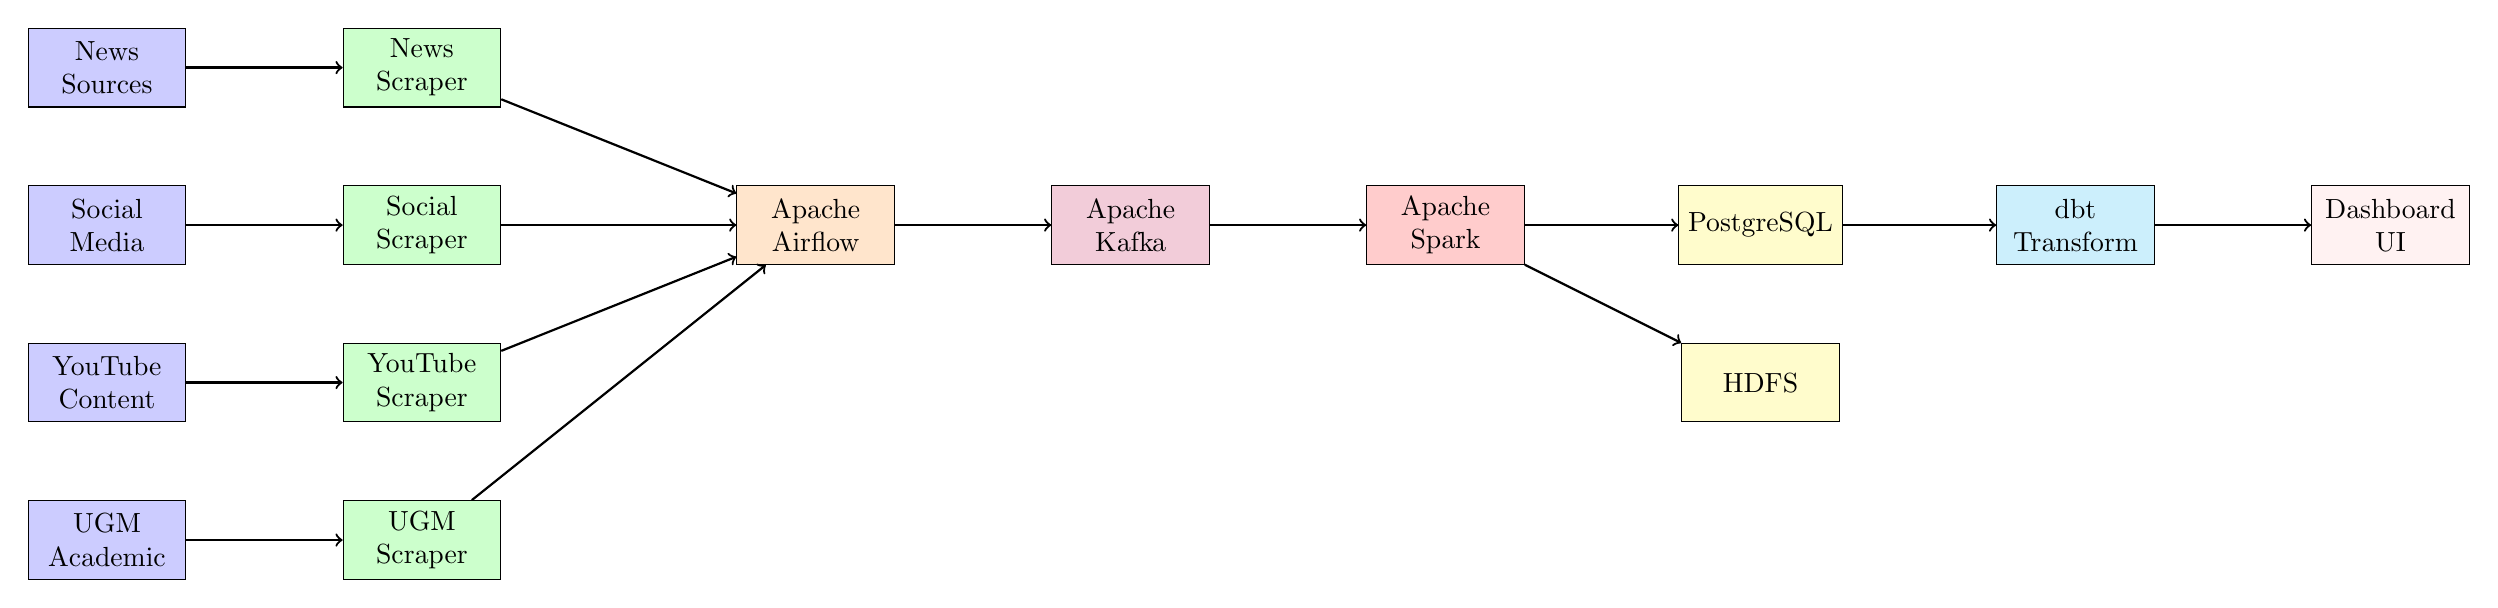
\begin{tikzpicture}[
    node distance=2cm,
    box/.style={rectangle, draw, minimum width=2cm, minimum height=1cm, align=center},
    arrow/.style={->, thick}
]
    % Data Sources
    \node[box, fill=blue!20] (ds1) {News\\Sources};
    \node[box, fill=blue!20, below of=ds1] (ds2) {Social\\Media};
    \node[box, fill=blue!20, below of=ds2] (ds3) {YouTube\\Content};
    \node[box, fill=blue!20, below of=ds3] (ds4) {UGM\\Academic};
    
    % Scrapers
    \node[box, fill=green!20, right of=ds1, xshift=2cm] (s1) {News\\Scraper};
    \node[box, fill=green!20, right of=ds2, xshift=2cm] (s2) {Social\\Scraper};
    \node[box, fill=green!20, right of=ds3, xshift=2cm] (s3) {YouTube\\Scraper};
    \node[box, fill=green!20, right of=ds4, xshift=2cm] (s4) {UGM\\Scraper};
    
    % Airflow
    \node[box, fill=orange!20, right of=s2, xshift=3cm] (af) {Apache\\Airflow};
    
    % Kafka
    \node[box, fill=purple!20, right of=af, xshift=2cm] (k) {Apache\\Kafka};
    
    % Spark
    \node[box, fill=red!20, right of=k, xshift=2cm] (sp) {Apache\\Spark};
    
    % Storage
    \node[box, fill=yellow!20, right of=sp, xshift=2cm] (pg) {PostgreSQL};
    \node[box, fill=yellow!20, below of=pg] (hdfs) {HDFS};
    
    % dbt
    \node[box, fill=cyan!20, right of=pg, xshift=2cm] (dbt) {dbt\\Transform};
    
    % Dashboard
    \node[box, fill=pink!20, right of=dbt, xshift=2cm] (ui) {Dashboard\\UI};
    
    % Arrows
    \draw[arrow] (ds1) -- (s1);
    \draw[arrow] (ds2) -- (s2);
    \draw[arrow] (ds3) -- (s3);
    \draw[arrow] (ds4) -- (s4);
    \draw[arrow] (s1) -- (af);
    \draw[arrow] (s2) -- (af);
    \draw[arrow] (s3) -- (af);
    \draw[arrow] (s4) -- (af);
    \draw[arrow] (af) -- (k);
    \draw[arrow] (k) -- (sp);
    \draw[arrow] (sp) -- (pg);
    \draw[arrow] (sp) -- (hdfs);
    \draw[arrow] (pg) -- (dbt);
    \draw[arrow] (dbt) -- (ui);
    
\end{tikzpicture}
\caption{System Architecture Overview}
\label{fig:architecture}
\end{figure}

\subsection{Technology Stack}

\begin{table}[H]
\centering
\begin{tabular}{|l|l|l|}
\hline
\textbf{Component} & \textbf{Technology} & \textbf{Purpose} \\
\hline
Data Collection & Python Scrapers & Web scraping and API integration \\
\hline
Workflow Orchestration & Apache Airflow & Pipeline scheduling and monitoring \\
\hline
Stream Processing & Apache Kafka & Real-time data ingestion \\
\hline
Data Processing & Apache Spark & Batch and stream processing \\
\hline
Storage & PostgreSQL + HDFS & Relational and distributed storage \\
\hline
Data Transformation & dbt & SQL-based transformations \\
\hline
Containerization & Docker \& Docker Compose & Service orchestration \\
\hline
Dashboard & Streamlit & Real-time data visualization \\
\hline
\end{tabular}
\caption{Technology Stack Overview}
\label{tab:tech-stack}
\end{table}

\section{Infrastructure Components}

\subsection{Containerized Services}
The system is fully containerized using Docker Compose, providing the following services:

\begin{lstlisting}[language=bash, caption=Docker Compose Services]
services:
  # HDFS Components
  namenode:      # HDFS NameNode (Port 9870)
  datanode:      # HDFS DataNode (Port 9864)
  resourcemanager: # YARN ResourceManager (Port 8088)
  nodemanager:   # YARN NodeManager (Port 8042)
  
  # Data Processing
  spark:         # Apache Spark (Port 8080)
  kafka:         # Apache Kafka (Port 9092)
  zookeeper:     # Kafka coordination (Port 2181)
  
  # Workflow Orchestration
  airflow:       # Airflow Web Server (Port 8081)
  airflow-scheduler: # Airflow Scheduler
  
  # Database
  postgres:      # PostgreSQL (Port 5432)
  
  # Monitoring
  kafka-ui:      # Kafka UI (Port 8083)
\end{lstlisting}

\subsection{Service Access Points}

\begin{table}[H]
\centering
\begin{tabular}{|l|l|l|}
\hline
\textbf{Service} & \textbf{URL} & \textbf{Purpose} \\
\hline
Airflow & http://localhost:8081 & Workflow orchestration \\
\hline
Kafka UI & http://localhost:8083 & Stream monitoring \\
\hline
Spark UI & http://localhost:8080 & Job monitoring \\
\hline
HDFS NameNode & http://localhost:9870 & File system management \\
\hline
YARN & http://localhost:8088 & Resource management \\
\hline
PostgreSQL & localhost:5432 & Database access \\
\hline
Dashboard & http://localhost:8501 & Data visualization \\
\hline
\end{tabular}
\caption{Service Access Points}
\label{tab:service-access}
\end{table}

\section{Data Pipeline Flow}

\subsection{Pipeline Overview}
The data pipeline operates on a 4-hour schedule and follows this sequence:

\begin{enumerate}
    \item \textbf{Data Collection}: Parallel execution of all scrapers
    \item \textbf{Data Validation}: Quality checks and validation
    \item \textbf{Data Storage}: Backup to HDFS and PostgreSQL
    \item \textbf{Data Processing}: Spark-based analysis and transformation
    \item \textbf{Analytics Update}: dbt transformations and dashboard refresh
    \item \textbf{Notification}: Completion status reporting
\end{enumerate}

\subsection{Detailed Pipeline Stages}

\subsubsection{1. Data Collection Stage}
\begin{itemize}
    \item \textbf{News Scraper}: Collects articles from Kompas, Detik, NewsAPI, GNews
    \item \textbf{Social Media Scraper}: Gathers posts from Reddit and Twitter
    \item \textbf{YouTube Scraper}: Extracts video data from WHO, CDC, and academic channels
    \item \textbf{UGM Scraper}: Collects academic content from Universitas Gadjah Mada
\end{itemize}

\subsubsection{2. Data Validation Stage}
\begin{itemize}
    \item Content quality assessment
    \item Duplicate detection
    \item Data completeness validation
    \item Schema compliance checking
\end{itemize}

\subsubsection{3. Data Storage Stage}
\begin{itemize}
    \item Raw data backup to HDFS
    \item Structured data storage in PostgreSQL
    \item Metadata management
\end{itemize}

\subsubsection{4. Data Processing Stage}
\begin{itemize}
    \item Sentiment analysis using NLP
    \item Topic classification and keyword extraction
    \item Data aggregation and summarization
    \item Real-time stream processing
\end{itemize}

\subsubsection{5. Analytics Stage}
\begin{itemize}
    \item dbt model execution
    \item Star schema population
    \item Analytics table generation
    \item Dashboard data refresh
\end{itemize}

\section{Data Model and Schema}

\subsection{Star Schema Design}
The system implements a star schema data warehouse with the following structure:

\begin{figure}[H]
\centering
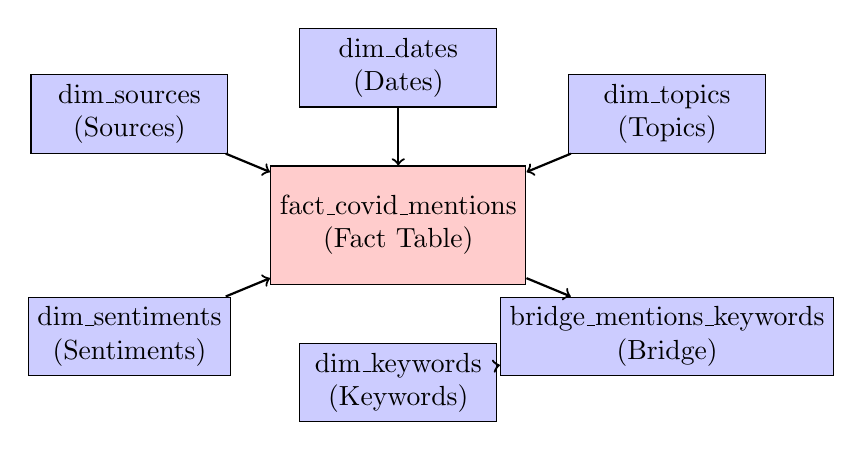
\begin{tikzpicture}[
    node distance=2cm,
    fact/.style={rectangle, draw, fill=red!20, minimum width=3cm, minimum height=1.5cm, align=center},
    dim/.style={rectangle, draw, fill=blue!20, minimum width=2.5cm, minimum height=1cm, align=center},
    arrow/.style={->, thick}
]
    % Fact Table
    \node[fact] (fact) {fact\_covid\_mentions\\(Fact Table)};
    
    % Dimension Tables
    \node[dim, above left of=fact, xshift=-2cm] (dim1) {dim\_sources\\(Sources)};
    \node[dim, above of=fact] (dim2) {dim\_dates\\(Dates)};
    \node[dim, above right of=fact, xshift=2cm] (dim3) {dim\_topics\\(Topics)};
    \node[dim, below left of=fact, xshift=-2cm] (dim4) {dim\_sentiments\\(Sentiments)};
    \node[dim, below of=fact] (dim5) {dim\_keywords\\(Keywords)};
    
    % Bridge Table
    \node[dim, below right of=fact, xshift=2cm] (bridge) {bridge\_mentions\_keywords\\(Bridge)};
    
    % Arrows
    \draw[arrow] (dim1) -- (fact);
    \draw[arrow] (dim2) -- (fact);
    \draw[arrow] (dim3) -- (fact);
    \draw[arrow] (dim4) -- (fact);
    \draw[arrow] (fact) -- (bridge);
    \draw[arrow] (dim5) -- (bridge);
    
\end{tikzpicture}
\caption{Star Schema Data Model}
\label{fig:star-schema}
\end{figure}

\subsection{Core Tables}

\subsubsection{Fact Table}
\begin{lstlisting}[language=sql, caption=Fact Table Schema]
CREATE TABLE fact_covid_mentions (
    id SERIAL PRIMARY KEY,
    source_id INTEGER REFERENCES dim_sources(id),
    date_id INTEGER REFERENCES dim_dates(id),
    topic_id INTEGER REFERENCES dim_topics(id),
    sentiment_id INTEGER REFERENCES dim_sentiments(id),
    title TEXT,
    content TEXT,
    url TEXT,
    engagement_score INTEGER,
    created_at TIMESTAMP DEFAULT NOW()
);
\end{lstlisting}

\subsubsection{Dimension Tables}
\begin{itemize}
    \item \textbf{dim\_sources}: Source information (name, type, platform)
    \item \textbf{dim\_dates}: Date dimensions (date, day, month, year, quarter)
    \item \textbf{dim\_topics}: Topic categories and classifications
    \item \textbf{dim\_sentiments}: Sentiment labels and score ranges
    \item \textbf{dim\_keywords}: Keyword information and weights
\end{itemize}

\subsubsection{Analytics Tables}
The system generates several analytics tables for dashboard consumption:
\begin{itemize}
    \item \textbf{fct\_bar\_chart\_data}: Source distribution analytics
    \item \textbf{fct\_line\_chart\_data}: Time series trend data
    \item \textbf{fct\_pie\_chart\_data}: Sentiment distribution
    \item \textbf{fct\_word\_cloud\_data}: Keyword frequency analysis
    \item \textbf{fct\_daily\_summary}: Daily aggregated metrics
    \item \textbf{rpt\_content\_overview}: Content overview reporting
\end{itemize}

\section{Data Processing and Analytics}

\subsection{Spark Processing Jobs}
The system includes several Spark-based processing jobs:

\begin{lstlisting}[language=python, caption=Spark Job Structure]
# Main processing jobs
backend/processing/jobs/
├── etl_batch.py           # Batch ETL processing
├── preprocessing.py       # Data preprocessing
└── spark_topic_sentiment.py  # Topic and sentiment analysis
\end{lstlisting}

\subsection{Key Processing Features}
\begin{itemize}
    \item \textbf{Sentiment Analysis}: NLP-based sentiment scoring
    \item \textbf{Topic Classification}: COVID-19 topic identification
    \item \textbf{Keyword Extraction}: Automatic keyword identification
    \item \textbf{Data Deduplication}: Duplicate content removal
    \item \textbf{Quality Scoring}: Content quality assessment
\end{itemize}

\subsection{dbt Transformations}
The system uses dbt for data transformation with the following model structure:

\begin{lstlisting}[language=sql, caption=dbt Model Structure]
models/
├── staging/           # Raw data staging
├── intermediate/      # Intermediate transformations
└── marts/
    ├── analytics/     # Analytics models
    ├── dimensions/    # Dimension tables
    └── reporting/     # Reporting models
\end{lstlisting}

\section{Dashboard and Visualization}

\subsection{Dashboard Features}
The real-time dashboard provides comprehensive COVID-19 data visualization:

\begin{itemize}
    \item \textbf{Key Metrics}: Total mentions, daily counts, sentiment scores
    \item \textbf{Interactive Charts}: Line, bar, pie charts with real-time updates
    \item \textbf{Word Cloud}: Keyword frequency visualization
    \item \textbf{Real-time Stream}: Live data feed
    \item \textbf{Responsive Design}: Mobile and desktop compatible
\end{itemize}

\subsection{Dashboard Components}

The COVID-19 Real-time Dashboard consists of several main components arranged hierarchically as follows:

\begin{enumerate}
    \item \textbf{Dashboard Header} \\
    The main title: \textit{COVID-19 Real-time Dashboard}.
    
    \item \textbf{Main Metrics Row} \\
    Consists of four key metrics displayed horizontally:
    \begin{itemize}
        \item \textbf{Total Mentions}: Displays the total number of COVID-19-related mentions.
        \item \textbf{Today's Mentions}: Displays the number of mentions that occurred today.
        \item \textbf{Average Sentiment}: Shows the average sentiment value from all mentions.
        \item \textbf{Active Sources}: Shows the number of active data sources.
    \end{itemize}
    
    \item \textbf{Daily Trend} \\
    A \textit{Line Chart} that shows the trend of COVID-19 mentions per day.
    
    \item \textbf{Source and Sentiment Distribution} \\
    Consists of two charts displayed side by side:
    \begin{itemize}
        \item \textbf{Bar Chart}: Shows the distribution of mentions by data source (e.g., news, social media, YouTube, etc.).
        \item \textbf{Pie Chart}: Shows the distribution of sentiment (positive, negative, neutral) from all mentions.
    \end{itemize}
    
    \item \textbf{Popular Keywords} \\
    A \textit{Word Cloud} that displays the most frequently occurring keywords or topics in the mention data.
    
    \item \textbf{Real-time Data Stream} \\
    Displays the latest mention data stream in real time, allowing users to monitor live data updates.
\end{enumerate}

\section{Monitoring and Operations}

\subsection{Airflow Monitoring}
The system provides comprehensive monitoring through Apache Airflow:

\begin{itemize}
    \item \textbf{DAG Monitoring}: Real-time pipeline status
    \item \textbf{Task Logs}: Detailed execution logs
    \item \textbf{Performance Metrics}: Execution time tracking
    \item \textbf{Error Handling}: Automatic retry mechanisms
    \item \textbf{Alerting}: Failure notifications
\end{itemize}

\subsection{Data Quality Monitoring}
\begin{itemize}
    \item \textbf{Automated Validation}: Data quality checks
    \item \textbf{Quality Metrics}: Completeness, accuracy, consistency
    \item \textbf{Error Reporting}: Detailed error logs
    \item \textbf{Performance Tracking}: Processing time monitoring
\end{itemize}

\section{Performance and Scalability}

\subsection{Performance Optimizations}
\begin{itemize}
    \item \textbf{Parallel Processing}: Concurrent scraper execution
    \item \textbf{Distributed Storage}: HDFS for large-scale data
    \item \textbf{Indexing}: Database query optimization
    \item \textbf{Caching}: Frequently accessed data caching
    \item \textbf{Resource Management}: YARN-based resource allocation
\end{itemize}

\subsection{Scalability Features}
\begin{itemize}
    \item \textbf{Horizontal Scaling}: Container-based deployment
    \item \textbf{Load Balancing}: Distributed processing
    \item \textbf{Fault Tolerance}: Automatic failover mechanisms
    \item \textbf{Data Partitioning}: Efficient data distribution
\end{itemize}

\section{Deployment and Configuration}

\subsection{Environment Setup}
The system requires the following environment variables:

\begin{lstlisting}[language=bash, caption=Environment Configuration]
# API Keys
NEWSAPI_KEY=your_newsapi_key
GNEWS_API_KEY=your_gnews_api_key
YOUTUBE_API_KEY=your_youtube_api_key

# Database Configuration
POSTGRES_HOST=localhost
POSTGRES_PORT=5432
POSTGRES_DB=risetdb
POSTGRES_USER=admin
POSTGRES_PASSWORD=admin

# Timezone Configuration
TZ=Asia/Jakarta
\end{lstlisting}

\subsection{Deployment Commands}
\begin{lstlisting}[language=bash, caption=Deployment Instructions]
# Start all services
docker-compose up -d

# Run scrapers manually
cd backend/scrapers
python main.py --mode run

# Execute dbt transformations
cd backend/dbt
dbt run

# Start dashboard
cd frontend/dashboard
python app.py
\end{lstlisting}

\section{Outputs and Deliverables}

\subsection{Primary Outputs}
\begin{enumerate}
    \item \textbf{Real-time Dashboard}: Interactive COVID-19 data visualization
    \item \textbf{Analytics Reports}: Automated reporting and insights
    \item \textbf{Data Warehouse}: Structured data for analysis
    \item \textbf{API Endpoints}: Data access interfaces
    \item \textbf{Monitoring Dashboards}: System health monitoring
\end{enumerate}

\subsection{Data Insights}
The system provides the following types of insights:
\begin{itemize}
    \item \textbf{Trend Analysis}: COVID-19 mention trends over time
    \item \textbf{Sentiment Analysis}: Public sentiment towards COVID-19
    \item \textbf{Source Analysis}: Content distribution across sources
    \item \textbf{Keyword Analysis}: Most discussed COVID-19 topics
    \item \textbf{Geographic Analysis}: Regional content distribution
\end{itemize}

\section{Conclusion}

The Big Data Research System represents a comprehensive solution for COVID-19 data collection, processing, and analysis. The system successfully integrates multiple data sources, implements robust data processing pipelines, and provides real-time analytics through an interactive dashboard.

Key achievements include:
\begin{itemize}
    \item \textbf{End-to-end Automation}: Complete data pipeline automation
    \item \textbf{Scalable Architecture}: Containerized, distributed system
    \item \textbf{Real-time Processing}: Live data streaming and analysis
    \item \textbf{Data Quality Assurance}: Comprehensive validation and monitoring
    \item \textbf{User-friendly Interface}: Interactive dashboard for data exploration
\end{itemize}

The system demonstrates modern big data best practices and provides a solid foundation for COVID-19 research and monitoring. The modular architecture allows for easy extension and modification to accommodate new data sources and analysis requirements.

\section{Future Enhancements}

Potential areas for future development include:
\begin{itemize}
    \item \textbf{Machine Learning Integration}: Advanced predictive analytics
    \item \textbf{Real-time Alerting}: Automated alert systems
    \item \textbf{API Development}: RESTful APIs for external access
    \item \textbf{Advanced Analytics}: Deep learning-based content analysis
    \item \textbf{Multi-language Support}: International content processing
\end{itemize}

\end{document} 